\documentclass[a4paper,12pt]{extarticle}
\usepackage[utf8x]{inputenc}
\usepackage[T1,T2A]{fontenc}
\usepackage[russian]{babel}
\usepackage{hyperref}
\usepackage{indentfirst}
\usepackage{listings}
\usepackage{color}
\usepackage{here}
\usepackage{array}
\usepackage{multirow}
\usepackage{graphicx}

\usepackage{caption}
\renewcommand{\lstlistingname}{Программа} % заголовок листингов кода

\bibliographystyle{ugost2008ls}

\usepackage{listings}
\lstset{ %
extendedchars=\true,
keepspaces=true,
language=C,						% choose the language of the code
basicstyle=\footnotesize,		% the size of the fonts that are used for the code
numbers=left,					% where to put the line-numbers
numberstyle=\footnotesize,		% the size of the fonts that are used for the line-numbers
stepnumber=1,					% the step between two line-numbers. If it is 1 each line will be numbered
numbersep=5pt,					% how far the line-numbers are from the code
backgroundcolor=\color{white},	% choose the background color. You must add \usepackage{color}
showspaces=false				% show spaces adding particular underscores
showstringspaces=false,			% underline spaces within strings
showtabs=false,					% show tabs within strings adding particular underscores
frame=single,           		% adds a frame around the code
tabsize=2,						% sets default tabsize to 2 spaces
captionpos=t,					% sets the caption-position to top
breaklines=true,				% sets automatic line breaking
breakatwhitespace=false,		% sets if automatic breaks should only happen at whitespace
escapeinside={\%*}{*)},			% if you want to add a comment within your code
postbreak=\raisebox{0ex}[0ex][0ex]{\ensuremath{\color{red}\hookrightarrow\space}},
texcl=true,
inputpath=listings,                     % директория с листингами
}

\usepackage[left=2cm,right=2cm,
top=2cm,bottom=2cm,bindingoffset=0cm]{geometry}

%% Нумерация картинок по секциям
\usepackage{chngcntr}
\counterwithin{figure}{section}
\counterwithin{table}{section}

%%Точки нумерации заголовков
\usepackage{titlesec}
\titlelabel{\thetitle.\quad}
\usepackage[dotinlabels]{titletoc}

%% Оформления подписи рисунка
\addto\captionsrussian{\renewcommand{\figurename}{Рисунок}}
\captionsetup[figure]{labelsep = period}

%% Подпись таблицы
\DeclareCaptionFormat{hfillstart}{\hfill#1#2#3\par}
\captionsetup[table]{format=hfillstart,labelsep=newline,justification=centering,skip=-10pt,textfont=bf}

%% Путь к каталогу с рисунками
\graphicspath{{fig/}}


\begin{document}	% начало документа

% Титульная страница
\begin{titlepage}	% начало титульной страницы

	\begin{center}		% выравнивание по центру

		\large Санкт-Петербургский Политехнический Университет Петра Великого\\
		\large Институт компьютерных наук и технологий \\
		\large Кафедра компьютерных систем и программных технологий\\[6cm]
		% название института, затем отступ 6см
		
		\huge Сети и телекоммуникации\\[0.5cm] % название работы, затем отступ 0,5см
		\large Отчет по лабораторной работе\\[0.1cm]
		\large Изучение сокетов и разработка собственных клиент-серверных приложений на сырых сокетах\\[5cm]

	\end{center}


	\begin{flushright} % выравнивание по правому краю
		\begin{minipage}{0.25\textwidth} % врезка в половину ширины текста
			\begin{flushleft} % выровнять её содержимое по левому краю

				\large\textbf{Работу выполнил:}\\
				\large Беседин Д.С.\\
				\large {Группа:} 43501/3\\
				
				\large \textbf{Преподаватель:}\\
				\large Алексюк А.О.

			\end{flushleft}
		\end{minipage}
	\end{flushright}
	
	\vfill % заполнить всё доступное ниже пространство

	\begin{center}
	\large Санкт-Петербург\\
	\large \the\year % вывести дату
	\end{center} % закончить выравнивание по центру

\thispagestyle{empty} % не нумеровать страницу
\end{titlepage} % конец титульной страницы

\vfill % заполнить всё доступное ниже пространство


% Содержание
% Содержание
\renewcommand\contentsname{\centerline{Содержание}}
\tableofcontents
\newpage




\section{Цель работы}
Целью работы являются изучение основных функций для работы с сокетами со стороны клиента и сервера, а также разработать собственный протокол взаимодействия и создать клиент-серверное приложение, работающего согласно разработанному протоколу.

\section{Программа работы}

\begin{enumerate}
\item Простейшее TCP клиент-серверное приложение
\begin{itemize}
\item Простейший эхо-сервер
\item Многопоточный TCP сервер
\end{itemize}

\item Простейшее UDP клиент-серверное приложение
\begin{itemize}
\item Простейший эхо-сервер
\end{itemize}

\item Разработка TCP приложения по индивидуальному заданию
\begin{itemize}
\item Индивидуальное задание
\item Разработка протокола взаимодействия
\item Написание многопоточного TCP сервера на ОС Linux
\item Написание клиента на ОС Windows
\end{itemize}

\item Разработка UDP приложения по индивидуальному заданию
\begin{itemize}
\item Индивидуальное задание
\item Разработка протокола взаимодействия
\item Написание UDP сервера на ОС Windows
\item Написание клиента на ОС Linux
\end{itemize}

\item Дополнительное задание
\begin{itemize}
\item Описание задания
\item Выполнение задания
\end{itemize}
\end{enumerate}

\section{Ход выполнения работы}

\subsection{Простейшее TCP клиент-серверное приложение}

\subsubsection{Простейший эхо-сервер}

Для разработки данного приложения необходимо изучить функции работы с сокетами на С.

Для создания сокета применяется функция:
\begin{lstlisting}
int socket(int domain, int type, int protocol);
\end{lstlisting}

Домен определяет пространство адресов, в котором располагается сокет, и множество протоколов, которые используются для передачи данных. Чаще других используются домены Unix и Internet, задаваемые константами AF\_UNIX и AF\_INET соответственно (префикс AF означает "address family" - "семейство адресов"). При задании AF\_UNIX для передачи данных используется файловая система ввода/вывода Unix. В этом случае сокеты используются для межпроцессного взаимодействия на одном компьютере и не годятся для работы по сети. Константа AF\_INET соответствует Internet-домену. Сокеты, размещенные в этом домене, могут использоваться для работы в любой IP-сети. Существуют и другие домены (AF\_IPX для протоколов Novell, AF\_INET6 для новой модификации протокола IP - IPv6 и т. д.).

Тип сокета определяет способ передачи данных по сети. Чаще других применяются:
\begin{itemize}
\item SOCK\_STREAM. Передача потока данных с предварительной установкой соединения. Обеспечивается надежный канал передачи данных, при котором фрагменты отправленного блока не теряются, не переупорядочиваются и не дублируются. Поскольку этот тип сокетов является самым распространенным, до конца раздела мы будем говорить только о нём. Остальным типам будут посвящены отдельные разделы.
\item SOCK\_DGRAM. Передача данных в виде отдельных сообщений (датаграмм). Предварительная установка соединения не требуется. Обмен данными происходит быстрее, но является ненадежным: сообщения могут теряться в пути, дублироваться и переупорядочиваться. Допускается передача сообщения нескольким получателям (multicasting) и широковещательная передача (broadcasting).
\item SOCK\_RAW. Этот тип присваивается низкоуровневым (т. н. "сырым") сокетам. Их отличие от обычных сокетов состоит в том, что с их помощью программа может взять на себя формирование некоторых заголовков, добавляемых к сообщению.
\end{itemize}
Для реализации SOCK\_STREAM используется протокол TCP, для реализации SOCK\_DGRAM - протокол UDP,

Прежде чем передавать данные через сокет, его необходимо связать с адресом в выбранном домене  с помощью функции:
\begin{lstlisting}
int bind(int sockfd, struct sockaddr *addr, int addrlen);
\end{lstlisting}
В качестве первого параметра передается дескриптор сокета, который мы хотим привязать к заданному адресу. Второй параметр, addr, содержит указатель на структуру с адресом, а третий - длину этой структуры.
Структура sockaddr иммет следующий вид:
\begin{lstlisting}
struct sockaddr {
    unsigned short    sa_family;    // Семейство адресов, AF\_xxx
    char              sa_data[14];  // 14 байтов для хранения адреса
};
\end{lstlisting}

Работать с этой структурой напрямую не очень удобно, поэтому будем использовать вместо sockaddr одну из альтернативных структур вида sockaddr\_XX (XX - суффикс, обозначающий домен: "un" - Unix, "in" - Internet и т. д.).При передаче в функцию bind указатель на эту структуру приводится к указателю на sockaddr. Рассмотрим для примера структуру sockaddr\_in:
\begin{lstlisting}
struct sockaddr_in {
    short int          sin_family;  // Семейство адресов
    unsigned short int sin_port;    // Номер порта
    struct in_addr     sin_addr;    // IP-адрес
    unsigned char      sin_zero[8]; // "Дополнение" до размера структуры sockaddr
};
\end{lstlisting}

На следующем шаге создается очередь запросов на соединение. При этом сокет переводится в режим ожидания запросов со стороны клиентов:
\begin{lstlisting}
int listen(int sockfd, int backlog);
\end{lstlisting}
Первый параметр - дескриптор сокета, а второй задает размер очереди запросов.

Когда сервер готов обслужить очередной запрос, он использует функцию accept:
\begin{lstlisting}
int accept(int sockfd, void *addr, int *addrlen);
\end{lstlisting}
Функция accept создает для общения с клиентом новый сокет и возвращает его дескриптор. Параметр sockfd задает слушающий сокет. После вызова он остается в слушающем состоянии и может принимать другие соединения. В структуру, на которую ссылается addr, записывается адрес сокета клиента, который установил соединение с сервером.

После того как соединение установлено, можно начинать обмен данными. Для этого используются функции send и recv в ОС Windows и read и write в ОС Linux:
\begin{lstlisting}
int send(int sockfd, const void *msg, int len, int flags);
int recv(int sockfd, const void *msg, int len, int flags);
\end{lstlisting}
Здесь sockfd - это, как всегда, дескриптор сокета, через который мы отправляем данные, msg - указатель на буфер с данными для send и буфер для приема данных для recv, len - длина буфера в байтах(сколько будет передано/считано), а flags - набор битовых флагов, управляющих работой функции.
\begin{lstlisting}
int write(int sockfd, const void *msg, int len);
int read(int sockfd, const void *msg, int len);
\end{lstlisting}
Функции для ОС Linux отличаются лишь отсутствием флагов.

Для закрытия сокета используются функции shutdown и close:
\begin{lstlisting}
int shutdown(int sockfd, int how);
int close(int fd);
\end{lstlisting}
С помощью shutdown можно закрыть сокет для передачи в каком-то направлении с помощью параметра how: 0 - запретить чтение, 1 - запретить запись, 2 - запретить и то и то.
Close() освобождает связанные с сокетом системные ресурсы.

С стороны клиента также установить соединение с сокетом, который будет открыт командой accept() сервера. Для этого используется функция connect:
\begin{lstlisting}
int connect(int sockfd, struct sockaddr *serv\_addr, int addrlen);
\end{lstlisting}
Здесь sockfd - сокет, который будет использоваться для обмена данными с сервером, serv\_addr содержит указатель на структуру с адресом сервера, а addrlen - длину этой структуры.

Порядок вызовов функций для работы с сокетами на стороне эхо-сервера:
\begin{itemize}
\item socket() - создает сокет
\item bind() - привязка созданного сокета к заданным IP-адресам и портам
\item listen() - переводит сокет в состояние прослушивания
\item accept() - принимает поступающие запросы на подключение и возвращает сокет для нового соединения
\item recv() - чтение данных от клиента из сокета, возвращенного на предыдущем шаге
\item send() - отправка только что принятых данных клиенту
\item shutdown() - разрыв соединения с клиентом
\item close() - для закрытия клиентского и слушающего сокетов
\end{itemize}

Порядок вызовов функций для работы с сокетами на стороне клиента:
\begin{itemize}
\item socket() - создает сокет
\item connect() - установка соединения для сокета, который будет связан с серверным сокетом, порожденным вызовом accept()
\item send() - отправка данных серверу
\item recv() - чтение тех же данных от сервера
\item shutdown() - разрыв соединения с клиентом
\item close() - для закрытия клиентского и слушающего сокетов
\end{itemize}

\subsubsection{Многопоточный TCP сервер}
Для организации работы сервера с множеством клиентов необходимо сделать следующее:
\begin{itemize}
\item Вынести общение с клиентом (send и recv) в отдельную функцию для того, чтобы была возможность вызывать ее в новом потоке.
\item Организовать работу функций listen() и accept() в цикле.
listen() должен работать с первым слушающий сокетом, а accept каждый раз будет создавать новый сокет для общения с клиентом.
\item Открывать новый поток, вызывая функцию общения с клиентом.
В функцию общения с клиентом необходимо передавать новый сокет, дескриптор которого возвращает accept.
\end{itemize}
Написанная функция общения с клиентом:
\begin{lstlisting}
void* readAndWrite (void* temp);
\end{lstlisting}
Функция принимает в качестве аргумента ссылку на дескриптор сокета. Возвращаемый результат void* и тип аргумента void * необходимы для вызова функции в новом потоке.
Преобразование аргумента в целочисленный дескриптор происходит следующим образом:
\begin{lstlisting}
int sock = *((int *) temp);
\end{lstlisting}

Вызов функций listen() и accept() выполнен в цикле:
\begin{lstlisting}
while(1){
        listen(sockfd, 5);
        newsockfd = accept(sockfd, (struct sockaddr *) &cli_addr, &(sizeof(cli_addr)));
	.....
}
\end{lstlisting}

После открытия нового сокета создается поток. В качестве аргументов ему передается функция работы с клиентом как стартовая функция работы потока, а также дескриптор сокета, чтобы его получила функция общения с клиентом. Создание такого потока на примере сервера на ОС Linux:
\begin{lstlisting}
while(1){
	....
        pthread_t tid;
        pthread_attr_t attr;
        pthread_attr_init(&attr);
        pthread_create(&tid, &attr,  readAndWrite, &newsockfd);
        pthread_detach(tid);
}
\end{lstlisting}
Использовались POSIX потоки.

\subsection{Простейший UDP клиент-сервер}
Для организации обмена через UDP и обмена с помощью датаграмм необходимо внести следующие изменения в функцию создания сокета, изменить функции чтения и записи, а также изменить порядок вызовов функций.

При создании сокетов как на стороне сервера, так и на стороне клиента, необходимо вторым аргументом (тип данных) передать константу SOCK\_DGRAM, для организации передачи датаграммами без подтверждения соединения.

Также при передаче через UDP изменятся функции чтения и передачи сообщений:
\begin{lstlisting}
ssize_t recvfrom(int sockfd, void *buf, size_t len, int flags, struct sockaddr *src_addr, socklen_t *addrlen);
ssize_t sendto(int sockfd, const void *buf, size_t len, int flags, const struct sockaddr *dest_addr, socklen_t addrlen);
\end{lstlisting}
В качестве аргументов передаются дескриптор сокета, буфер для чтения/записи, флаги. структура с информацией о передающей/принимабщей стороне, длина этой структуры.
Возвращаемое значение - число реально принятых/переданных символов.

Изменится и состав вызова функций для работы с сокетами на клиенте и сервере. 
Порядок действий сервера:
\begin{itemize}
\item socket() - создает сокет
\item bind() - привязка созданного сокета к заданным IP-адресам и портам
\item recfromv() - чтение данных от клиента из сокета, возвращенного на предыдущем шаге
\item sendto() - отправка только что принятых данных клиенту
\item shutdown() - разрыв соединения с клиентом
\item close() - для закрытия клиентского и слушающего сокетов
\end{itemize}
Для организации обмена по UDP не происходит прослушивание сокетом на подключение и подтверждения соединения с созданием нового сокета.

Порядок действий клиента:
\begin{itemize}
\item socket() - создает сокет
\item connect() - установка соединения для сокета, который будет связан с серверным сокетом, порожденным вызовом accept()
\item senfrom() - отправка данных серверу
\item recvto() - чтение тех же данных от сервера
\item shutdown() - разрыв соединения с клиентом
\item close() - для закрытия клиентского и слушающего сокетов
\end{itemize}
Действия клиента не меняются, однако возможно не использовать подтверждение соединения с помощью connect()

\subsection{Разработка TCP приложения по индивидуальному заданию}
\subsubsection{Индивидуальное задание}
Необходимо разработать приложение для обмена файлами, основанное на протоколе FTP. Реализуемые функции:
\begin{itemize}
\item ls - получение содержимого текущего каталога
\item cd - смена текущей директории
\item pull - передача файла от сервера клиенту
\item push - передача файла от клиента на сервер
\end{itemize}

Сначала необходимо разработать собственный протокол взаимодействия клиента и сервера. Далее необходимо написать клиент-серверное приложение (Сервер на ОС Linux, клиент на ОС Windows), работающее согласно разработанному протоколу и реализующее заданную функциональность.
\subsubsection{Разработка протокола взаимодействия}
После подключения клиента к серверу, второй начинает ожидать присланной ему команды от клиента. Соответственно клиент имеет 4 возможные команды, которые считываются из консоли, куда их вводит пользователь. Пользователь вводит команду следующего вида:
\begin{lstlisting}
<command> <argument>
\end{lstlisting}
В качестве команд применяются строки "ls", "cd, "pull", "push". Далее, после пробела, следует аргумент. Аргументом может служить путь к директории от текущего положения клиента (для команд ls и cd), имя файла (для pull и push). После ввода команды в консоль, приложение клиента запускает процедуру распарсивания полученной строки для получения аргумента и определения, какая команда была введена. Если введенная команда не совпадает ни с одной из 4-х возможных, то выводится сообщение "Unknown command", и приложение ждет ввода новой команды. Если было обнаружено совпадение с одной из возможных команд, то вызывается функция общения с сервером. Далее представлено взаимодействие клиента и сервера друг с другом при вводе различных команд.

\begin{itemize}
\item Команда получения содержимого текущего каталога ls
\end{itemize}

Клиент составляет команду для отправки ее на сервер. Для этого в пустую строку в 256 зарезервированных символов заносится сама команда с пробелом после ("ls "), затем к ней приписывается полный путь к текущему каталогу, в котором находится клиент на сервере, затем без пробелов приписывается введенный пользователем аргумент. Далее серверу отправляется сообщение длинною в 3 символа, в котором в строчном виде записана длина полученной команды. Сервер, принимая это сообщение, переводит полученную строку и целочисленной значение и ждет приема сообщения указанной длины. Клиент посылает команду серверу и начинает ждать ответного сообщения длиною в 1 символ. 

После приема самой команды, на стороне сервера также запускается распарсивание, в ходе которого сервер отделяет аргумент от команды, и вызывает функцию для обработки команды ls. Сервер делает попытку открыть директорию по указанному в аргументе пути, записывая в строку для ответа клиенту "n" при неудачной попытке отрыть каталог и "y" при успешной. Далее сервер посылает клиенту это сообщение длиной в 1 символ. 

Клиент принимает от сервера подтверждение ("y") или отказ ("n"). В случае отказа функция завершается и приложение снова ждет ввода команды от пользователя. В случае подтверждения клиент начинает в цикле принимать сообщения по 256 символов. Условием окончания приема становится принятая строка "\_end\_of\_ls".

Сервер же, после отправки подтверждения, начинает в цикле получать по одному имена файлов и директорий открытого каталога, записывать из в строку и отправлять клиенту по 256 символов за одно сообщение. После перебора всего содержимого сервер отправляет строку "\_end\_of\_ls" и переходит в режим принятия следующей команды.

\begin{itemize}
\item Команда смены текущей директории каталога cd
\end{itemize}

Клиент составляет полную команду для посылки серверу по тому же алгоритму, что и в команде ls (в качестве команды с пробелом используется строка "cd "). Далее клиент отправляет серверу сообщение в 3 символа, в котором содержится длина получившейся команды, а затем и саму команду. После клиент переходит в режим ожидания подтверждения: ожидает прием сообщения длиною в один символ.

Сервер, после получения сообщения с длиной команды, принимает команду указанной длины и обрабатывает ее. Сервер делает попытку открыть директорию, указанную в аргументе, и составляет сообщение-ответ: "n" при неудачной попытке открытия и "y" при успешном открытии. Это сообщение отправляется клиенту. Сервер завершает обработку команды и переходит в режим ожидания следующей команды.

Клиент, после приема сообщения проверяет его: если принят символ "y", то текущая директория меняется согласно указанному пользователем аргументу (либо приписывается новый каталог, либо (если аргумент "..") стирается последний каталог). 

\begin{itemize}
\item Команда взятия файла с сервера pull
\end{itemize}

Клиент делает попытку создать файл с указанным именем и открыть его. В случае неудачи выводится ошибка и клиент не совершает никакого обмена с сервером. Если же файл был успешно создан, то клиент составляет команду по алгоритму выше, но в качестве команды использует строку "pull ". Также отправляется длина полученной полной команды, а затем и сама команда. Клиент переходит в состояния ожидания подтверждения или отказа.

Сервер после принятия команды делает попытку открыть указанный в аргументе файл, и составляет сообщение-ответ: "n" при неудаче и "y" при успешном открытии файла. Данное сообщение отправляется клиенту.

Сервер после отправки подтверждения начинает читать открытый файл, максимум по 256 символов за одну итерацию цикла. Затем отправляется сообщение длиною в 3 символа, которое содержит кол-во считанных из файла символов. Далее отправляется сообщение, содержащее информацию, которую считали из файла. После окончания файла сервер посылает строку "\_end\_of\_file".

После получения подтверждения, клиент начинает в цикле прием сообщений от сервера. На каждой итерации цикла клиент принимает 2 сообщения: первое длиною в 3 символа содержит длину информационной посылки, второе - информационная посылка. После приема информационного сообщения оно записывается в файл. Условием окончания цикла является прием строки "\_end\_of\_file" в качестве информационного сообщения. 

\begin{itemize}
\item Команда записи файла на сервер push
\end{itemize}

Данная команда выполняется аналогично команде pull, но клиент и сервер меняются местами в основном цикле приема-передачи: клиент в цикле читает файл, отправляет длину считанных данных и отправляет данные, а сервер осуществляет прием и запись в файл, пока не получит строку "\_end\_of\_file".

\subsubsection{Написание многопоточного TCP сервера на ОС Linux}
Основная логика создания сокетов, привязка их к адресам, выделения новых потоков для общения с клиентами осталась такой же, как и в простейшем многопоточном эхо-сервере.

Изменилась функция общения с клиентом: теперь она содержит прием сразу двух сообщений подряд: длину команды и саму команду, после чего вызывает функцию парса, в которую передает принятую команду. 

Функция parse разделяет принятое сообщение на команду и аргумент, проверяет команду и вызывает функцию обработки команды:
\begin{lstlisting}
if (!(strncmp(command, "cd", 2))) direxist(sock, arg);
if (!(strncmp(command, "ls", 2))) ls(sock, arg);
if (!(strncmp(command, "pull", 4))) pull(sock, arg);
if (!(strncmp(command, "push", 4))) push (sock,arg);
\end{lstlisting}

Функции обработки действуют по описанным в протоколе алгоритмам:
\begin{itemize}
\item dirExist открывает каталог и отправляет сообщение с подтверждением или отказом.
\item ls открывает каталог, отправляет подтверждение, и отсылает содержимое в сообщениях по 256 байт.
\item pull открывает файл на чтение, отправляет подтверждение, читает файл по 256 байт и отправляет считанные данные, пока не прочтет весь файл, перед каждым сообщением отправляя размер текущей посылки. После окончания файла посылает сообщение-метку "\_end\_of\_file".
\item push создает файл для записи, отправляет подтверждение и начинает принимать сообщения о длине информационной посылки и саму информационную посылку, пока не будет принята метка об окончании файла. Каждое информационное сообщение записывается в созданный файл.
\end{itemize}

Для получения перевода целочисленного значения длины посылки в char[] была написана функция:
\begin{lstlisting}
char * makeStrFromInt (int len) {
    char buf[3];
    char * p = buf;
    int temp;
    p[2] = ((int)(len % 10) + '0');
    temp = len / 10;
    p[1] = ((int)(temp % 10) + '0');
    p[0] = ((int)(temp / 10) + '0');
    return p;
}
\end{lstlisting}

Также необходимо было учитывать, что в командах ls, pull и push используются метки для указания о завершении выполнения команды, а значит может существовать название файла или строка в файле, которые совпадут с этой меткой. Для этого была сделана функция экранирования:
\begin{lstlisting}
void pastShield (char * sendbuff) {
    for (int i = strnlen(sendbuff, 256) - 1; i >= 0; i--)
        sendbuff[i + 1] = sendbuff[i];
    sendbuff[0] = '/';
}
\end{lstlisting}
Если нам необходимо отправить информационную строку, которая совпадает с меткой, то вызывается эта функция.

Соответственно если было принято сообщение с "экраном", значит нам необходимо этот экран убрать:
\begin{lstlisting}
void deleteShield (char * str) {
    for (int i = 0; i < strnlen(str, 256) - 1; i++)
        str[i] = str[i + 1];
}
\end{lstlisting}

Для выполнения требования о возможности сервера отключать клиентов, а также отключаться полностью было добавлено следующее:
\begin{enumerate}
\item Массив сокетов
\item Массив флагов
\item Функция приема и обработки команд с серверной консоли
\item Вызов этой функции в отдельном потоке
\item Проверка флагов на отключение клиента в цикле работе с клиентом
\end{enumerate}

Массив сокетов - массив целых чисел, где хранятся дескрипторы сокетов всех подключенных клиентов.

Массив флагов - флаги для определения "свободных" ячеек массива сокетов, "занятых" и "посланных на отключение".

Функция приема сообщений с консоли сервера:
\begin{lstlisting}
void* servConsole(void* temp);
\end{lstlisting}
В качестве аргумента ей передается слушающий сокет сервера, т.к. отключение сервера предполагает закрытие этого сокета.
В этой функции осуществляется считывание строк с консоли, определяется, написана ли строка "exit" или "closeXXX". В случае exit и closeall осуществляется установка флагов всех клиентов в режим закрытия (exit также закрывает слушающий сокет). Если после "close" указан номер клиента, то функция установит флаг этого клиента в состояние закрытия.

Проверка флагов осуществляется каждым потоком перед принятием очередной команды. Таким образом, закрытие сокета клиента произойдет только после окончания текущего обмена.

Данная функция вызывается в отдельном потоке перед входом в цикл ожидания подключения новых клиентов.

\subsubsection{Написание клиента на ОС Windows}
Сетевая часть клиента также не отличается от простейшего TCP клиента. 
Также изменилась функция общения с сервером: она лишь получает введенную в консоль строку и запускает для нее процедуру parse.

Процедура парса также отделяет команду от аргумента и проверят, какая команда была введена, вызывая соответствующую функцию (если введенная команда не совпадает ни с одной из возможных, то функция возвращает константу UNKNOWN\_COMMAND, что приведет к выводу соответствующего сообщения в консоль).

Функции обработки введенных команд действуют по описанным в протоколе алгоритмам:
\begin{itemize}
\item dirChange (вызывается при команде cd) составляет команду, отправляет ее длину, отправляет команду и ждет подтверждения. В случае успешного открытия каталога на стороне сервера меняет текущий рабочего каталога.
\item ls составляет команду, отправляет ее длину и саму команду, после чего ждет подтверждения. В случае успешного открытия каталога на стороне сервера начинает прием посылок по 256 байт, выводя их в консоль, пока не будет принята посылка об окончании содержимого каталога.
\item pull создает файл для записи, составляет команду, отправляет ее длину и саму команду, после чего ждет подтверждения. После приема подтверждения начинает принимать сообщения о длине информационной посылки и саму информационную посылку, пока не будет принята метка об окончании файла. Каждое информационное сообщение записывается в созданный файл.
\item push открывает файл на чтение, составляет команду, отправляет ее длину и саму команду, после чего ждет подтверждения. При приеме подтверждения читает файл по 256 байт и отправляет считанные данные, пока не прочтет весь файл, перед каждым сообщением отправляя размер текущей посылки. После окончания файла посылает сообщение-метку "\_end\_of\_file".
\end{itemize}

Также как и в сервере здесь необходимы функции экранирования (pastShield и deleteShield) и перевода целого числа в char[].

Т.к. клиент в каждой функции обработки запроса должен составлять команду, то это действие было вынесено в отдельную функцию:
\begin{lstlisting}
int makePost(char * post, char * com, char * arg) {
    memset(post, 0, 256);
    strncat(post, com, strlen(com));
    strncat(post, addr, strlen(addr));
    strncat(post, arg, 256 - strlen(com) - strlen(arg));
    return 1;
}
\end{lstlisting}
Принимая указатели на строку для записи итоговой команды, строки, содержащие команду и аргумент, эта функция записывает в строку для итоговой команды саму команду с пробелом, затем полный путь к текущей директории, затем аргумент.

\subsection{Разработка UDP приложения по индивидуальному заданию}
\subsubsection{Индивидуальное задание}
Функциональные требования к приложению остались теми же, как и у TCP приложения. Отличие от TCP приложения: необходимо добавить контроль номера принятых и посланных пакетов, чтобы определить случаи потери или перемешивания пакетов.
\subsubsection{Разработка протокола взаимодействия}
Основные особенности протокола в формате и длине пакетов остались без изменений, однако для каждого отправленного пакета первые 2 байта резервируются для номера пакета. Таким образом, максимальная длина команд и данных для отправки становится 254 байта вместо 256.

\subsubsection{Написание UDP сервера}
UDP сервер был написан на основе TCP сервера, описанного выше. Отличия от TCP сервера:
\begin{enumerate}
\item Вызывать функцию работы с клиентами в основном потоке, т.к. нет необходимости в создании новых сокетов для клиентов. Все запросы от клиентов будут помещаться в очередь и обрабатываться последовательно. 
\item Вставлять в отправляемые пакеты их номер в текущей транзакции
\item Проверять номер принятых пакетов
\item Передавать в функции обработки команд данные о клиенте, с которым идет обмен сообщениями.
\end{enumerate}

Для работы с номерами пакетов были написаны 2 функции: для вставки номера пакета в сообщение и для проверки номера принятого пакета.
\begin{lstlisting}
void pastPacketNumber(char * post, int number, int len) {
    for (int i = len - 1; i > 1; i--) {
        post[i] = post[i-2];
    }
    post[0] = (int)(number / 10) + '0';
    post[1] = number % 10 + '0';
}
\end{lstlisting}
Функция принимает ссылку на сообщение, номер, который необходимо вставить в сообщение и длину сообщения. Функция "сдвигает" сообщение на 2 символа и в освободившиеся 2 байта вставляет номер пакета.

\begin{lstlisting}
int checkRec (char * mes, int counter) {
    char temp[2];
    temp[0] = mes[0];
    temp[1] = mes[1];
    for (int i = 0; i < strlen(mes); i++) {
        mes[i] = mes[i+2];
    }
    int co = atoi(temp);
    if (co == counter + 1) return 0;
    printf("Ошибка приема - неверный порядок пакетов\n");
    return 1;
}
\end{lstlisting}
Функция проверки номера принятого пакета принимает ссылку на буфер с принятым сообщением и номер пакета, уменьшенный на единицу. Осуществляется проверка номера принятого пакета и номер стирается из сообщения.

Также была изменена функция обработки команды на стороне сервера о завершении сервера. Данная функция просто осуществляет считывание команды с консоли и закрывает сокет, если была написана необходимая команда - "close".

\subsubsection{Написание UDP клиента}
UDP клиент также написан на основе TCP клиента. Однако также как и для сервера необходимо было добавить функции для вставки номера пакета в сообщения и проверки номера пакета в принятом сообщении. 

\subsection{Дополнительное задание}
\subsubsection{Описание задания}
Проанализировать код с помощью статического и динамического анализатора. Проверить код с помощью cppcheck, описать полученные ошибки и предупреждения, предложить вариант исправления. Также проанализировать работу программ на предмет утечки памяти с помощью утилиты valgrind.

\subsubsection{Выполнение задания}
Проверим исходный код TCP клиента по индивидуальному заданию с помощью cppcheck.
В ходе проверки программа выдала 6 предупреждений:
\begin{figure}[H]
	\begin{center}
		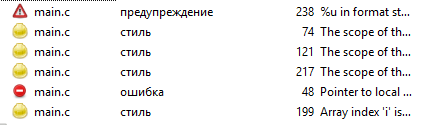
\includegraphics[scale=0.7]{cppcheck_tcpcli}
		\caption{Предупреждения от cppcheck для кода TCP клиента} 
		\label{pic:cppcheck1} % название для ссылок внутри кода
	\end{center}
\end{figure}

Результат содержит 4 стилистических предупреждения. 
3 из них указывают на то, что переменная, объявляемая в начале функции, инициализируется лишь после проверки условия и не используется вне участка кода, принадлежащему условию. Т.е. утилита говорит о том, что эту переменную можно объявлять уже после проверки условия, где она первый раз инициализируется. 
Последнее стилистическое предупреждение говорит о том, что в цикле for в качестве переменной для перебора используется переменная, которая была объявлена и использована до вызова for. Данной предупреждение исправить нельзя: в функции parse есть необходимость перебирать в цикле строку не с первого символа, а с того, на котором закончит предыдущий цикл, т.е. использовать ту же самую переменную.

Также присутствует одно предупреждение: в строке, выводимой в консоль, требуется указать переменную типа unsigned int, а на деле ей передается просто int переменная. Исправить легко: переделать выводимую строку так, чтобы она принимала int, или объявить переменную как unsigned int.

Последнее предупреждение cppcheck относится к ошибкам. Оно указывает на функцию получения строки в 3 символа из числа. Дело в том, что данная функция возвращает указатель на массив char, который создается внутри этой же функции. После выхода из функции данные в памяти могут быть стерты, что приведет к неверному возвращаемому значению. Решить это можно выделением памяти с помощью malloc или же передавая в функцию указатель, по которому будет записываться требуемое значение. Второй способ хуже тем, что в таком случае придется изменить способ применения функции во всей программе.

Проверим также UDP сервер:
\begin{figure}[H]
	\begin{center}
		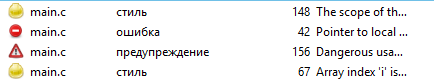
\includegraphics[scale=0.7]{cppcheck_udpcli}
		\caption{Предупреждения от cppcheck для кода UDP сервера} 
		\label{pic:cppcheck2} % название для ссылок внутри кода
	\end{center}
\end{figure}

Ошибка и 2 стилистических предупреждения совпадают с указанными выше, а вот предупреждение новое: оно отсылается к функции strncat, точнее к ее третьему аргументу. Предполагается, что третьим аргументом будет задано максимальное число байт для записи в строку, однако в данном месте кода в качестве третьего аргумента указана длина буфера, в который производится запись. Суть предупреждения в том, что если буфер был не пустой, то при записи максимального числа байт, которая начнется не с начала буфера, можно переписать участки памяти, располагающиеся за буфером. В данной программе это не приводит к ошибке, потому что данная запись производится в пустую строку и всегда начинается с нуля. Однако в общем случае можно в качестве третьего аргумента передавать максимальную длину массива, уменьшенную на число уже записанных в него символов (его фактическую длину).

Далее осуществим динамическую проверку на предмет утечек памяти с помощью утилиты valgrind. Для начала проверим многопоточный TCP сервер (подключимся клиентом к серверу и попробуем сделать каждую возможную операцию):
\begin{figure}[H]
	\begin{center}
		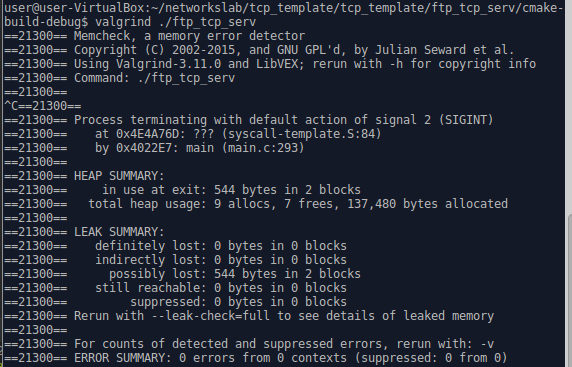
\includegraphics[scale=0.7]{valgrind_ftc_serv}
		\caption{Предупреждения от valgrind для кода TCP сервера} 
		\label{pic:valgr1} % название для ссылок внутри кода
	\end{center}
\end{figure}
Утилита показала отсутствие ошибок, но посоветовала запустить полную проверку с помощью ключа --leak-check=full. 
Итоги такой проверки:
\begin{figure}[H]
	\begin{center}
		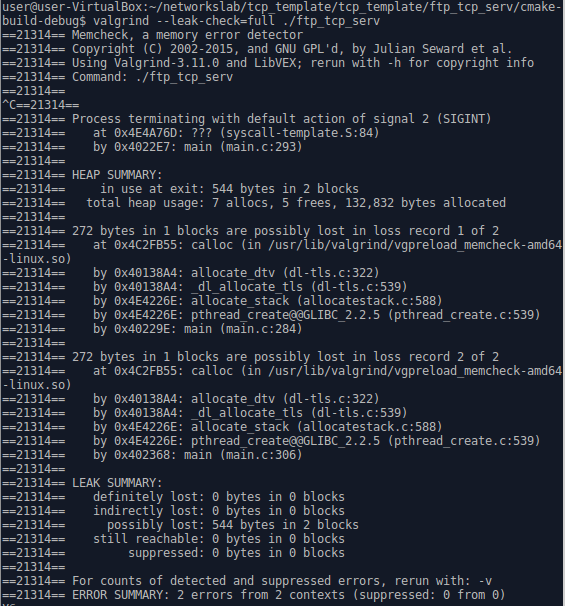
\includegraphics[scale=0.7]{valgrind_ftc_serv2}
		\caption{Предупреждения от valgrind для кода TCP сервера} 
		\label{pic:valgr2} % название для ссылок внутри кода
	\end{center}
\end{figure}
Видим, что при создании новых потоков может происходить потеря 272 байт информации. Вероятно это свзяано с тем, что в функцию начала работы потока передается дексриптор сокета как void*.

\section{Выводы}
В ходе выполнения работы были разработаны 2 клиент-серверных приложения для обмена файлами: на TCP и UDP сокетах. Приложения работали согласно заданию, реализуя разработанный протокол, а также отлавливая ошибки при работе с сетью: ошибки при создании сокетов, соединении, приеме и передаче информации. 

Стоит отметить, что в случае с TCP сокетом процедура создания соединения сложнее, чем в UDP, однако TCP обеспечивает контроль пакетов, что значительно облегчает нашу работу по написанию программы: нет необходимости контролировать пакеты на предмет утери или перемешивания.
Несмотря на то что мы лишь отслеживали случаи потери или перемешивания пакетов в UDP, не пытаясь исправлять данные ошибки, это значительно усложнило разработку и отладку приложения.

Однако в UDP приложении нет необходимости привязывать сокеты к адресам и выделять отдельный поток для каждого клиента. Это увеличивает скорость работы (обмены на основе UDP часто применяются там, где необходима скорость соединения), но усложняет контроль целостности данных. 

В качестве выводов также хочется сказать, что для приложения обмена файлами было удобнее использовать именно TCP сокеты, так как в данном случае очень важна именно целостность данных. Несмотря на то что UDP приложение также передает файлы без ошибок, на более удаленных друг от друга клиенте и сервере может происходить потеря и перемешивание пакетов, что приведет к неправильному приеме, а исправление таких ошибок, как и было указано выше, значительно усложняет разработку программы.

Также в ходе работы была применена работа с потоками. С их помощью было очень удобно разделить между собой работу с клиентами в случае TCP и обслуживание серверной консоли для TCP и UDP.
\end{document}
